\section{Liste: Alle Skateparks}
Auf der ersten Seite sollte man sofort einen Überblick über alle Skateparks erhalten, die wir in
unserer Datenbank gespeichert haben.

\begin{figure}[H]
  \begin{center}
    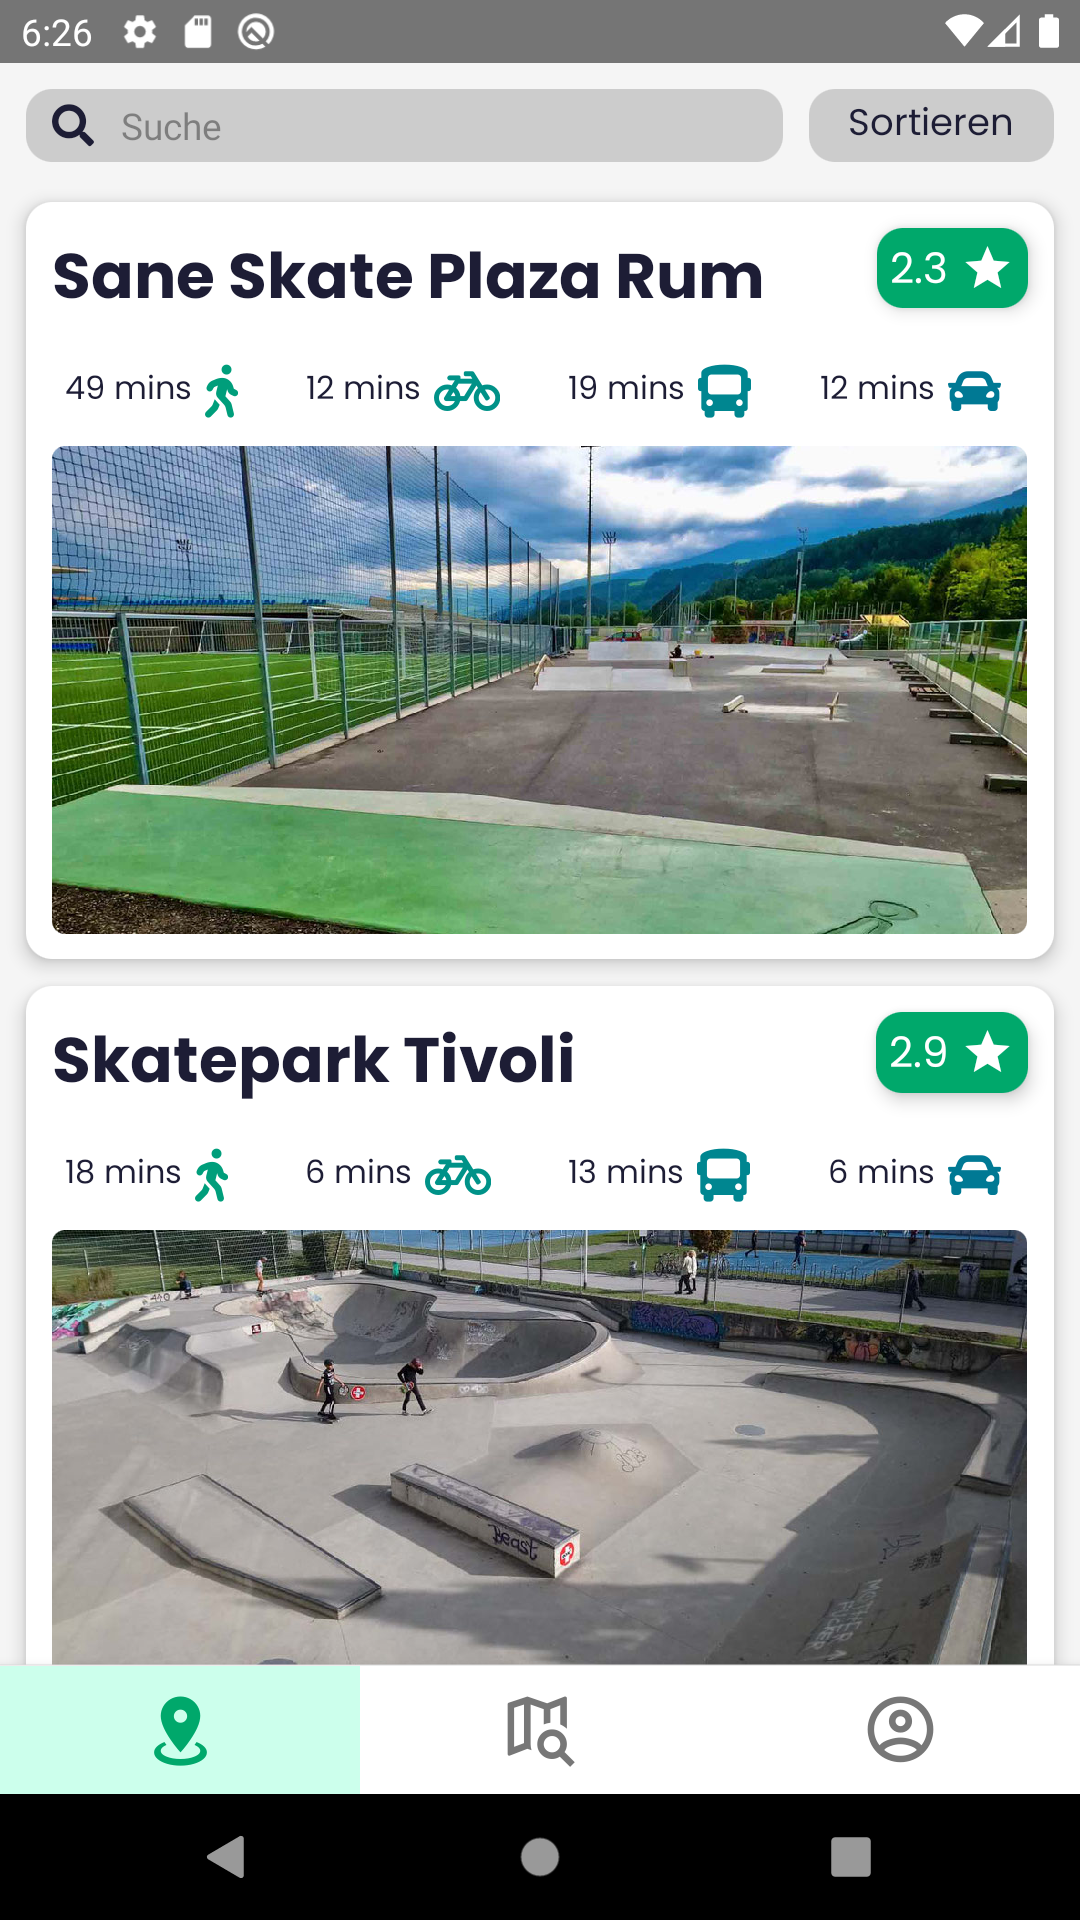
\includegraphics[width=0.5\textwidth]{Mobile/SkateparksList.png}
    \caption{SkateparksList Screen}
  \end{center}
\end{figure}

\subsection{Zusammensetzung}
\subsubsection{SkateparkEntry}
Ein einzelner Skatepark-Eintrag wird als SkateparkEntry dargestellt. Diese Komponente besteht aus
einem Header, Dauer bis zur Ankunft mit mehreren Fortbewegungsmitteln und einem Bild.

\begin{lstlisting}
  
\end{lstlisting}

